\documentclass{standalone}
\usepackage{pgfplots}

\begin{document}
\tikzset{every picture/.style={line width=0.75pt}} %set default line width to 0.75pt        
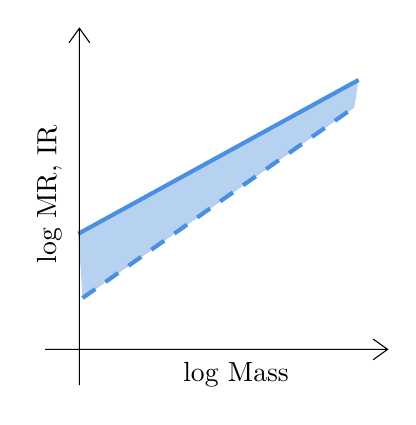
\begin{tikzpicture}[x=0.75pt,y=0.75pt,yscale=-1,xscale=1]
%uncomment if require: \path (0,219); %set diagram left start at 0, and has height of 219

%Shape: Polygon [id:ds9526223895836252] 
\draw  [draw opacity=0][fill={rgb, 255:red, 183; green, 209; blue, 240 }  ,fill opacity=1 ] (390,47.92) -- (388,61) -- (257,153) -- (255,122) -- (285,105.92) -- cycle ;
%Straight Lines [id:da8413299718907006] 
\draw [color={rgb, 255:red, 74; green, 144; blue, 226 }  ,draw opacity=1 ][fill={rgb, 255:red, 61; green, 139; blue, 230 }  ,fill opacity=1 ][line width=1.5]    (255,122) -- (390,47.92) ;


%Shape: Axis 2D [id:dp044209979443870395] 
\draw  (239,177.73) -- (404,177.73)(255.5,23) -- (255.5,194.92) (397,172.73) -- (404,177.73) -- (397,182.73) (250.5,30) -- (255.5,23) -- (260.5,30)  ;
%Straight Lines [id:da7008934539582028] 
\draw [color={rgb, 255:red, 74; green, 144; blue, 226 }  ,draw opacity=1 ][fill={rgb, 255:red, 61; green, 139; blue, 230 }  ,fill opacity=1 ][line width=1.5]  [dash pattern={on 5.63pt off 4.5pt}]  (257,153) -- (388,61) ;

% Text Node
\draw (331,190) node  [align=left] {log Mass};
% Text Node
\draw (241,103) node [rotate=-270.08] [align=left] {log MR, IR};


\end{tikzpicture}

\end{document}